\graphicspath{ {Figures/chapter02} }


This chapter describes the details of a mechanical BPS including a description of its mechanical parts, electrical and software that is used to control the system.

\section{Mechanical structure}
In order to balance a ball on a flat platform, there were several options and several designs that served this purpose, and each design had advantages and disadvantages that must be chosen between. Based on degree of freedom of the plate, Figure 2.1 demonstrate a different types of designs. to reduce the number of actuators and reduce the level of complexity in the platform, we chose the 2-DOF design since 2 is so enough to control the both axis of the plate.
To achieve this design six main parts was needed, the base, the joint, rods, servo holder, the plate and the ball.
\begin{figure}[h]
    \centering
    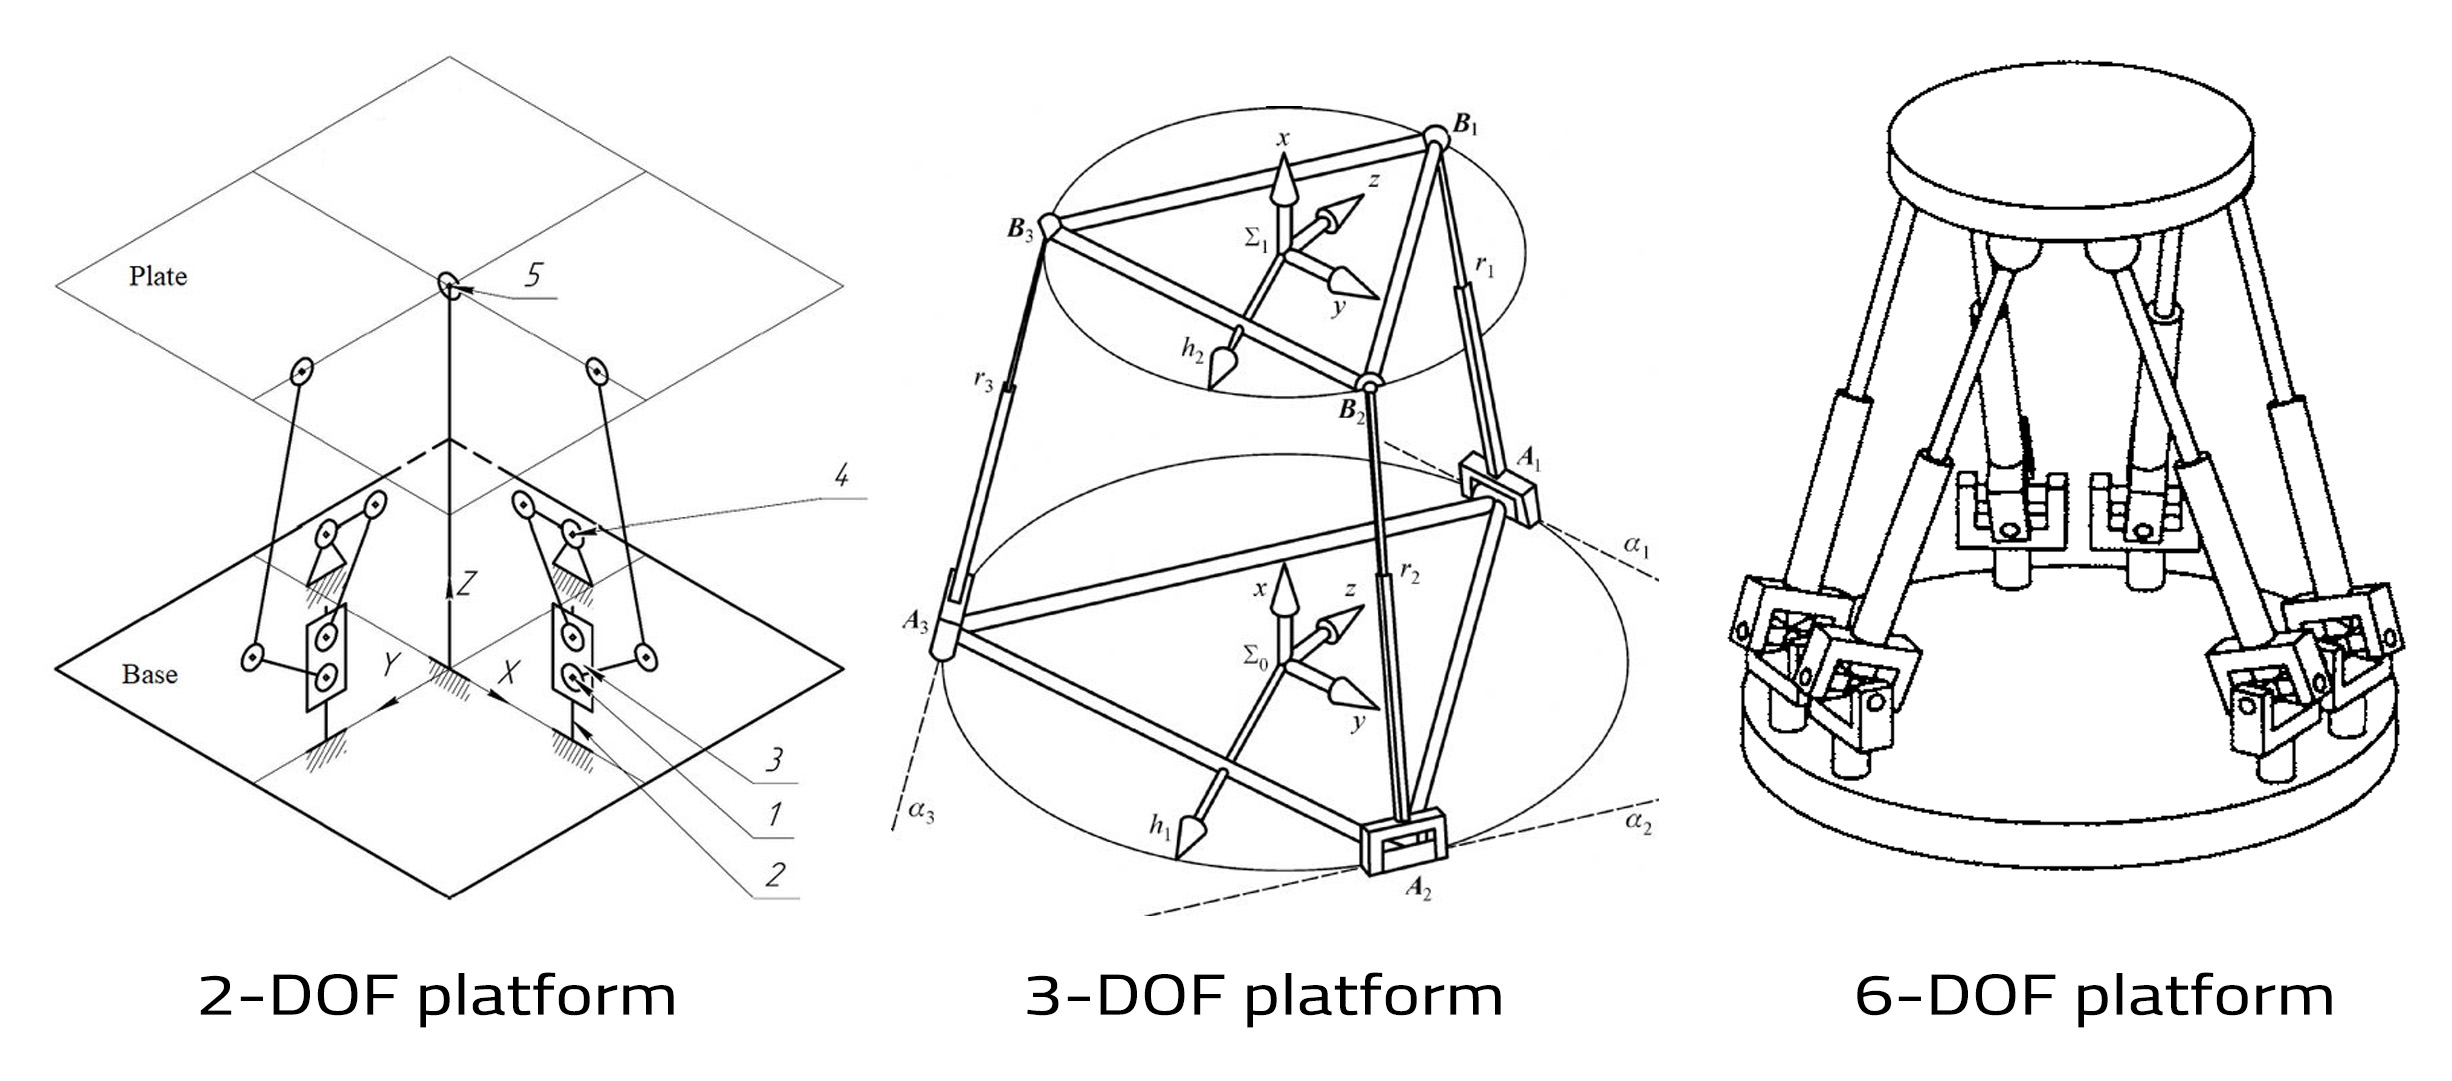
\includegraphics[width=1\linewidth]{DOF_Types_Platform.jpg}
    \caption{A variety of Ball and Plate System platform types based on the degree of freedom}
\end{figure}

\begin{itemize}
  \item \textbf{Base:} For the base a black rectangular piece of wood was selected with dimensions of 45 x 19.5 x 2 cm, this base serves as a main base on which the rest of the mechanical and electronic parts stand.
  
  \item \textbf{Joint:} the pivotal connection allowing the plate to move around two axes is crucial.Two types of joints were considered shown in figure 2.2: the universal joint and the ball joint. The ball joint was chosen for its superior flexibility, enabling smooth and responsive movements of the plate. This decision contributes to the overall adaptability and performance of the ball-on-plate system.
  
  \begin{figure}[h]
    \centering
    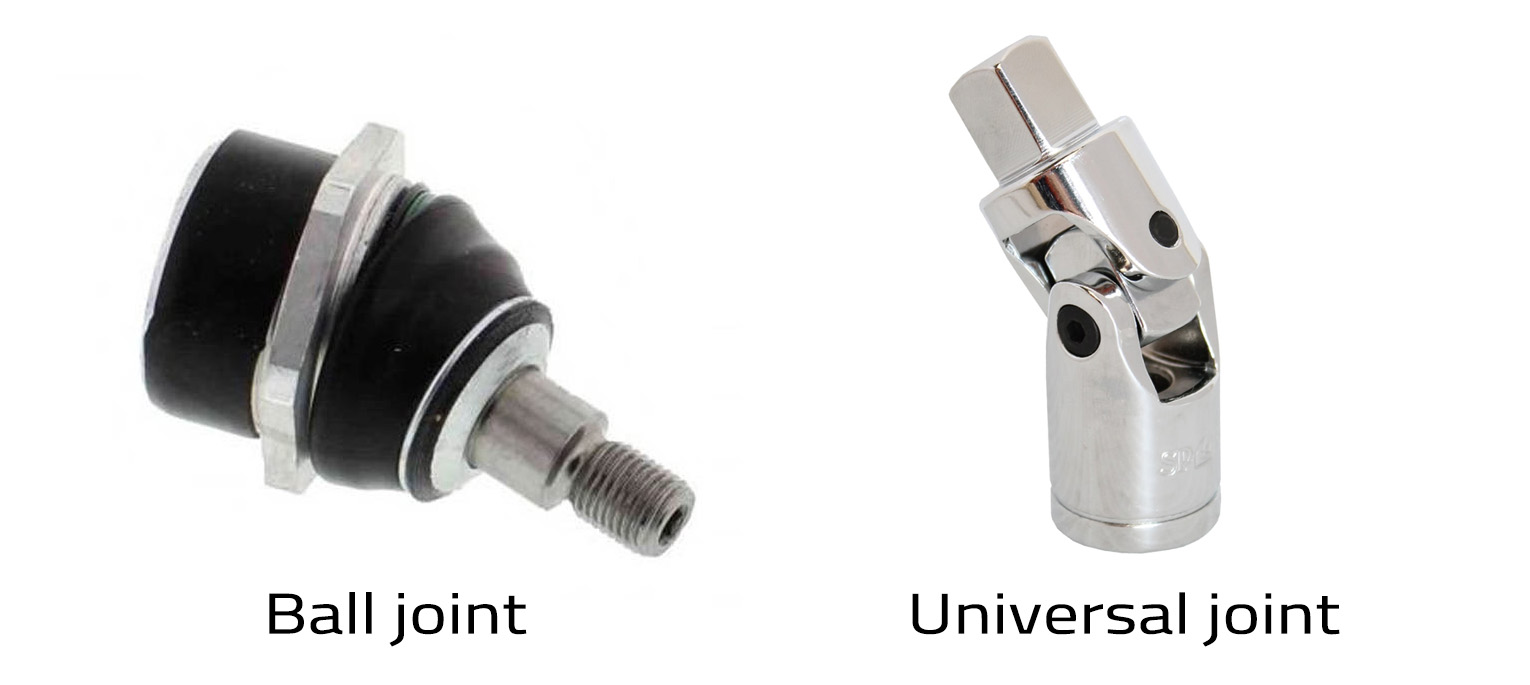
\includegraphics[width=0.9\linewidth]{joints.jpg}
    \caption{Two types of joints considered in the design - universal joint and ball joint}
    \label{fig:enter-label}
\end{figure}

  \item \textbf{Rods:} A linkage part between the servomotor and the plate that converts tho rotational movement into a linear motion, 20 degree at most of inclination is considered, so the angle relation with the dimension is analyzed and calculated in chapter 3
  
  \item \textbf{Servo Holder:} A simple aluminum structure that holds the servos in place, facilitating controlled movements and reduce the servomotor vibration, shown in figure 2.3.
  
\begin{figure}[h]
    \centering
    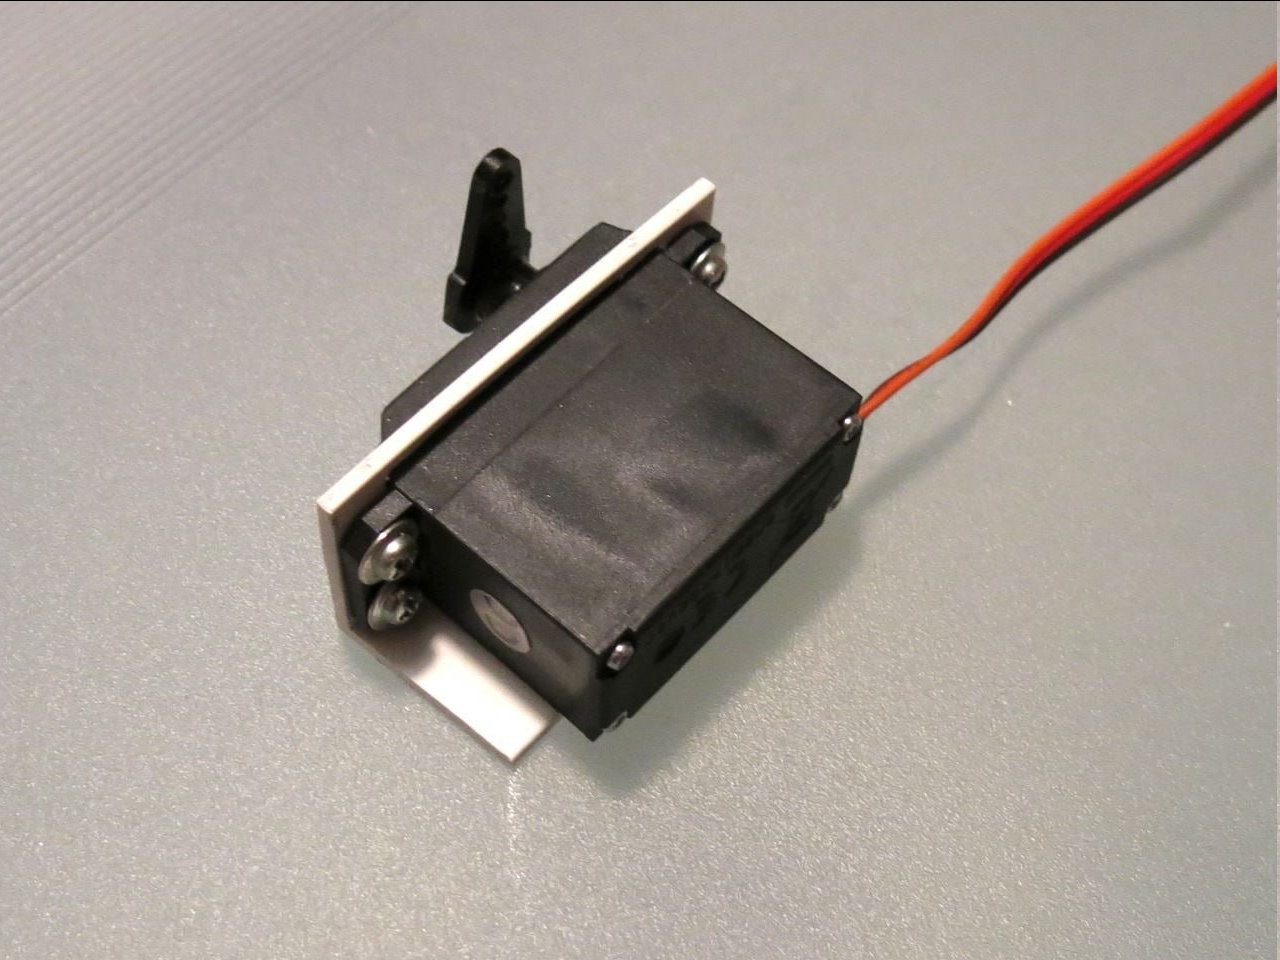
\includegraphics[width=0.55\linewidth]{Servomot_holder.png}
    \caption{The holder structure for the servomotor, ensuring controlled movements and reduced vibration}
    \label{fig:enter-label}
\end{figure}
  \item \textbf{Plate:} Transparent plastic flat platform where the ball rests.
  \item \textbf{Ball:} The object most be spherical symmetrical solid to be balanced on the plate , The ball’s mass should be not lower than 70 g. If the force is too small, two different effects can be observed: no touch is detected and the sensor returns Not a Number (NaN) signal or the ball is temporarily detected in a different place
\end{itemize}

\section{Electrical parts}
The circuit used and all the electrical parts are shown in figure 2.4
\begin{figure}[h]
    \centering
    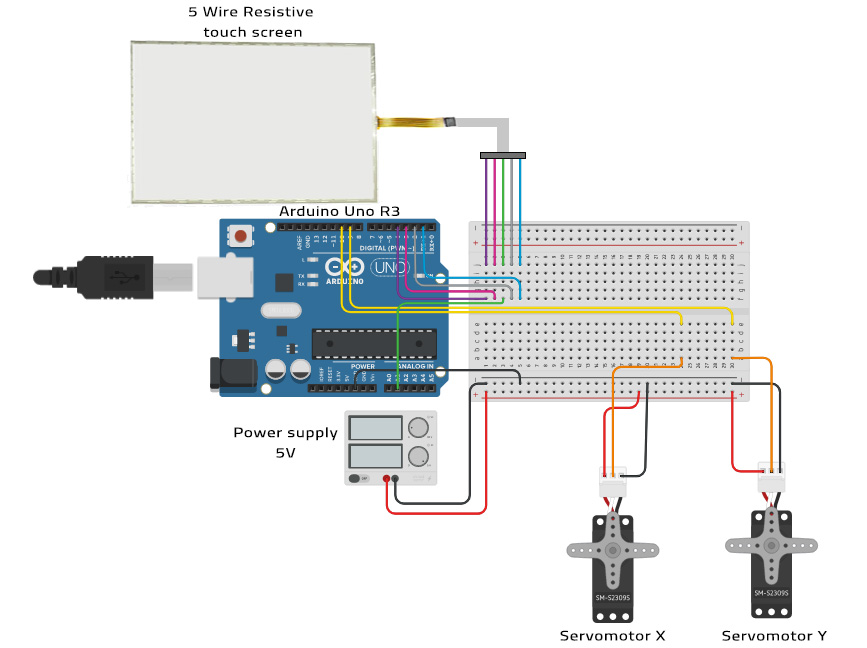
\includegraphics[width=1\linewidth]{Arduino_schematic.jpg}
    \caption{ Basic schematic illustrating the electrical components and circuitry of the System}
    \label{fig:enter-label}
\end{figure}
\subsection{Actuators}
For our 2-DOF plant, where the plate tilts around its center, two actuators are required to control tilt along the X and Y axes. Accuracy is crucial for achieving zero steady-state error. The Servo motor and stepper motor shown in figure 2.5 are the most suitable choices.\\
\begin{figure}[h]
    \centering
    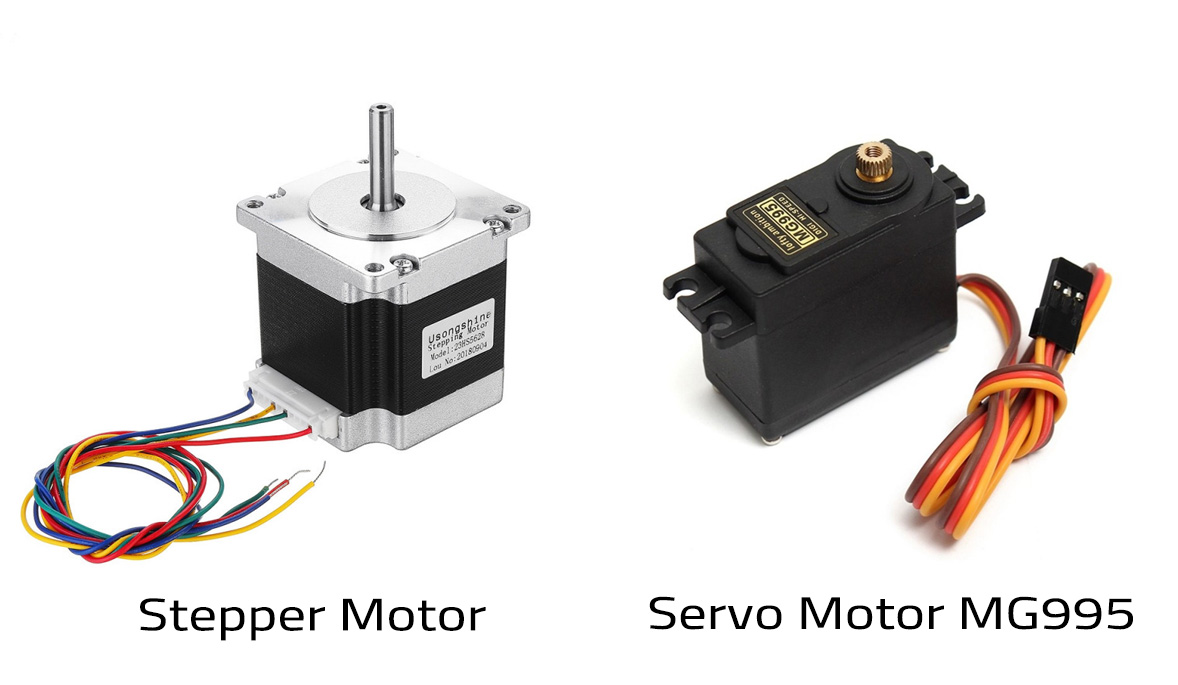
\includegraphics[width=0.75\linewidth]{Actuators_types.jpg}
    \caption{Types of actuators explored for the 2-DOF system - Stepper Motor and Servo Motor}
    \label{fig:enter-label}
\end{figure}

\textbf{Stepper Motor:}
\begin{itemize}
    \item Comes without an encoder or drive, requiring separate purchase, installation, and control.
    \item Relatively more expansive 
    \item Encoder feedback is used to eliminate missed steps.
    \item Torque decreases with speed, and steppers consume continuous current unless controlled not to.
\end{itemize}

\textbf{Servo Motor:}
\begin{itemize}
    \item DC motor with a gearbox for speed reduction and higher torque.
    \item Internal circuitry includes an encoder/potentiometer and controller.
    \item Powered by two cables and commanded via Pulse-width modulation(PWM).
    \item Consumes current only when needed, running cooler.
\end{itemize}

Servomotors are used as the actuators. The choice has been motivated by the fact that servos do not require the use of an additional control loop for engine rotation. Additionally, their relatively low cost is also an essential advantage. The servomotors are equipped with a proportional controller. The Pulse Width Modulation (PWM) signal is used to control them, the pulse cycle is equal to 20 ms and pulse width is in the 1000–2000 \(\mu\)s range. Their rotational range is \(60\deg\), the maximum speed is 0.5 s/\(60\deg\).
\subsection{Sensor}
In the BPS, achieving accurate ball location detection is fundamental for effective control. For this purpose, we explored various sensor options. While alternatives like cameras, infrared sensors, and capacitive systems are available, we went for resistive touch screens due to their versatility and cost-effectiveness. In particular, we have chosen the 17'' 5-wire resistive touch screen pad (Width of the panel was 355 mm, its height was 290 mm)

A five-wire resistive touchscreen, much like its four-wire counterpart, comprises two transparent resistive plates separated by insulating spacers. In this configuration, the top plate features a metalized contact, serving as the voltage sensing node. The bottom plate's four corners generate voltage gradients in both the x and y directions (refer to Figure 2.6).
\begin{figure}[h]
    \centering
    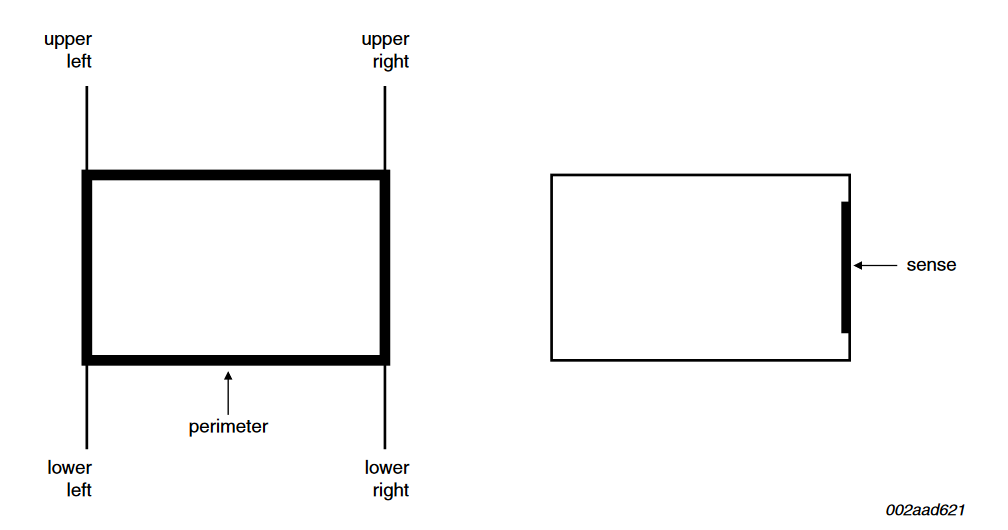
\includegraphics[width=1\linewidth]{structure_5_wire.png}
    \caption{Structure of 5-wire resistive touch screen}
    \label{fig:enter-label}
\end{figure}
The way the touchscreen works is by setting up specific ways for measuring both sideways (x-direction) and up-down (y-direction). When you press the screen with enough force, the top part bends and touches the bottom part. Figuring out the resistance in a 5-wire touchscreen can be a bit complex, but the addition of circuits along the edges of the touchscreen makes it simpler to think of it like a tool that divides voltage at the spot where it's touched. This, of course, depends on using the right setup called biasing.

Biasing the upper left and right corners to Vss and biasing the lower corners to Vdd enables measurement of the y-coordinate. Conversely, biasing the left side to Vss and the right side to Vdd facilitates measurement of the x-coordinate. Simultaneously biasing all four corners to Vss serves to detect when the screen is touched, triggering an interrupt (see Figure 2.7).
\begin{figure}[h]
    \centering
    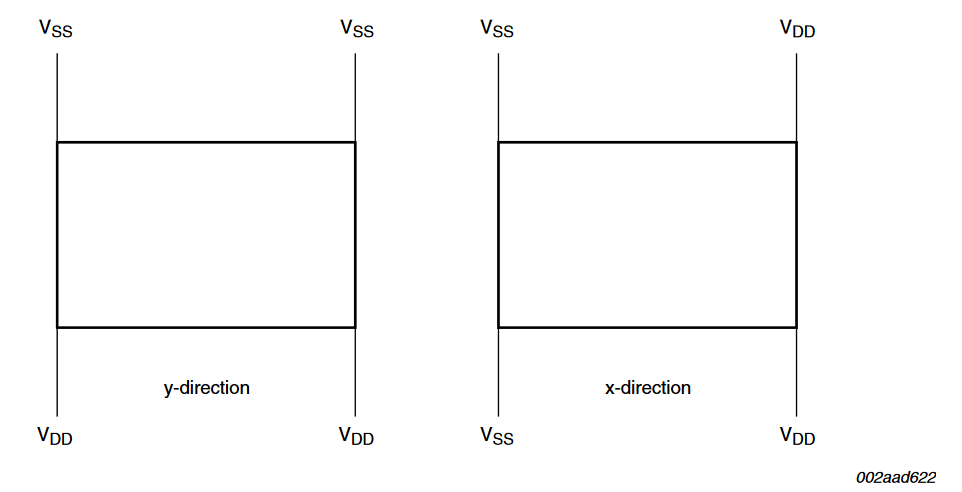
\includegraphics[width=1\linewidth]{Touchscreen_reaading.png}
    \caption{ Biasing setup for reading x and y directions of a 5-wire resistive touch screen}
    \label{fig:enter-label}
\end{figure}
In the touch condition, the sense signal from the screen connects to a port pin programmed as an input with a high resistance pullup. All corners of the touchscreen are driven to a logic zero. When touched, a voltage divider is established between the internal pullup of the port pin and the resistance of the touch screen. Notably, the resistance of the touch screen is significantly lower than the pullup connected to the sense signal. Consequently, when a touch occurs, the voltage at the sense signal pin approaches zero, initiating an interrupt.the biasing and measurement requirements for each of the four wires of the touchscreen are summarized in Table 2.1 .
\begin{table}[h]
\centering
\caption{Touchscreen interface requirements}
\label{tab:touchscreen_requirements}
\begin{tabular}{|p{2.5cm}|c|c|c|c|p{2cm}|}
\hline
\textbf{Function} & \textbf{Upper left} & \textbf{Lower left} & \textbf{Upper right} & \textbf{Lower right} & \textbf{Sense} \\ \hline
Hardware touch detection & Vss & Vss & Vss & Vss & Logic zero interrupt \\ \hline
Read x-position & Vss & Vss & V\tiny{DD} & V\tiny{DD} & Voltage measurement \\ \hline
Read y-position & Vss & V\tiny{DD} & Vss & V\tiny{DD} & Voltage measurement \\ \hline
\end{tabular}
\end{table}

The touch panel, while effective, has some disadvantages. It's highly sensitive to disturbances, requiring sufficient pressure into the plate, If the force of the touch is too small, two issues can arise: either no touch is detected, resulting in a NaN signal, or the touch is temporarily detected in a different location than its actual position. While these problems are rare when the ball is stationary, constant rolling can introduce measurement errors. Additionally, tilting the plate can reduce the gravity force component perpendicular to the plate, making the pressure force on the screen insufficient.

To mitigate these issues, several filters are employed:
\begin{enumerate}
    \item A filter detects when the sensor stops detecting the ball, and the touch panel returns invalid position values (zero, NaN or etc). When identified, the filter ignores these values, using the last meaningful number as the current position.
    \item lowpass filter that identifies high magnitude spikes when the sensor detects an incorrect ball position. If the current position change exceeds a certain threshold, it is ignored.
    \item An arithmetic filter collects n measurements of the ball position and calculates it as the sum of the measurements divided by n.(An average and median filters was considered to select in between).
\end{enumerate}

\subsection{Microcontroller}
In this work, two approaches to control the system was implemented, in the first approach Arduino Uno R3 was used as a microcontroller,Through it, the sensor data is retrieved and filtered, then through the same Arduino the PID signal is calculated and given to the servomotor as an output. in the second approach, the Arduino only played the role of data acquisition from the sensor to send it to the PC through a serial communication. The computer, using Simulink, processes the data, filters it, controls it, and sends the control signal to the Arduino again, which in turn sends it to the servo motor.
\begin{figure}[h]
    \centering
    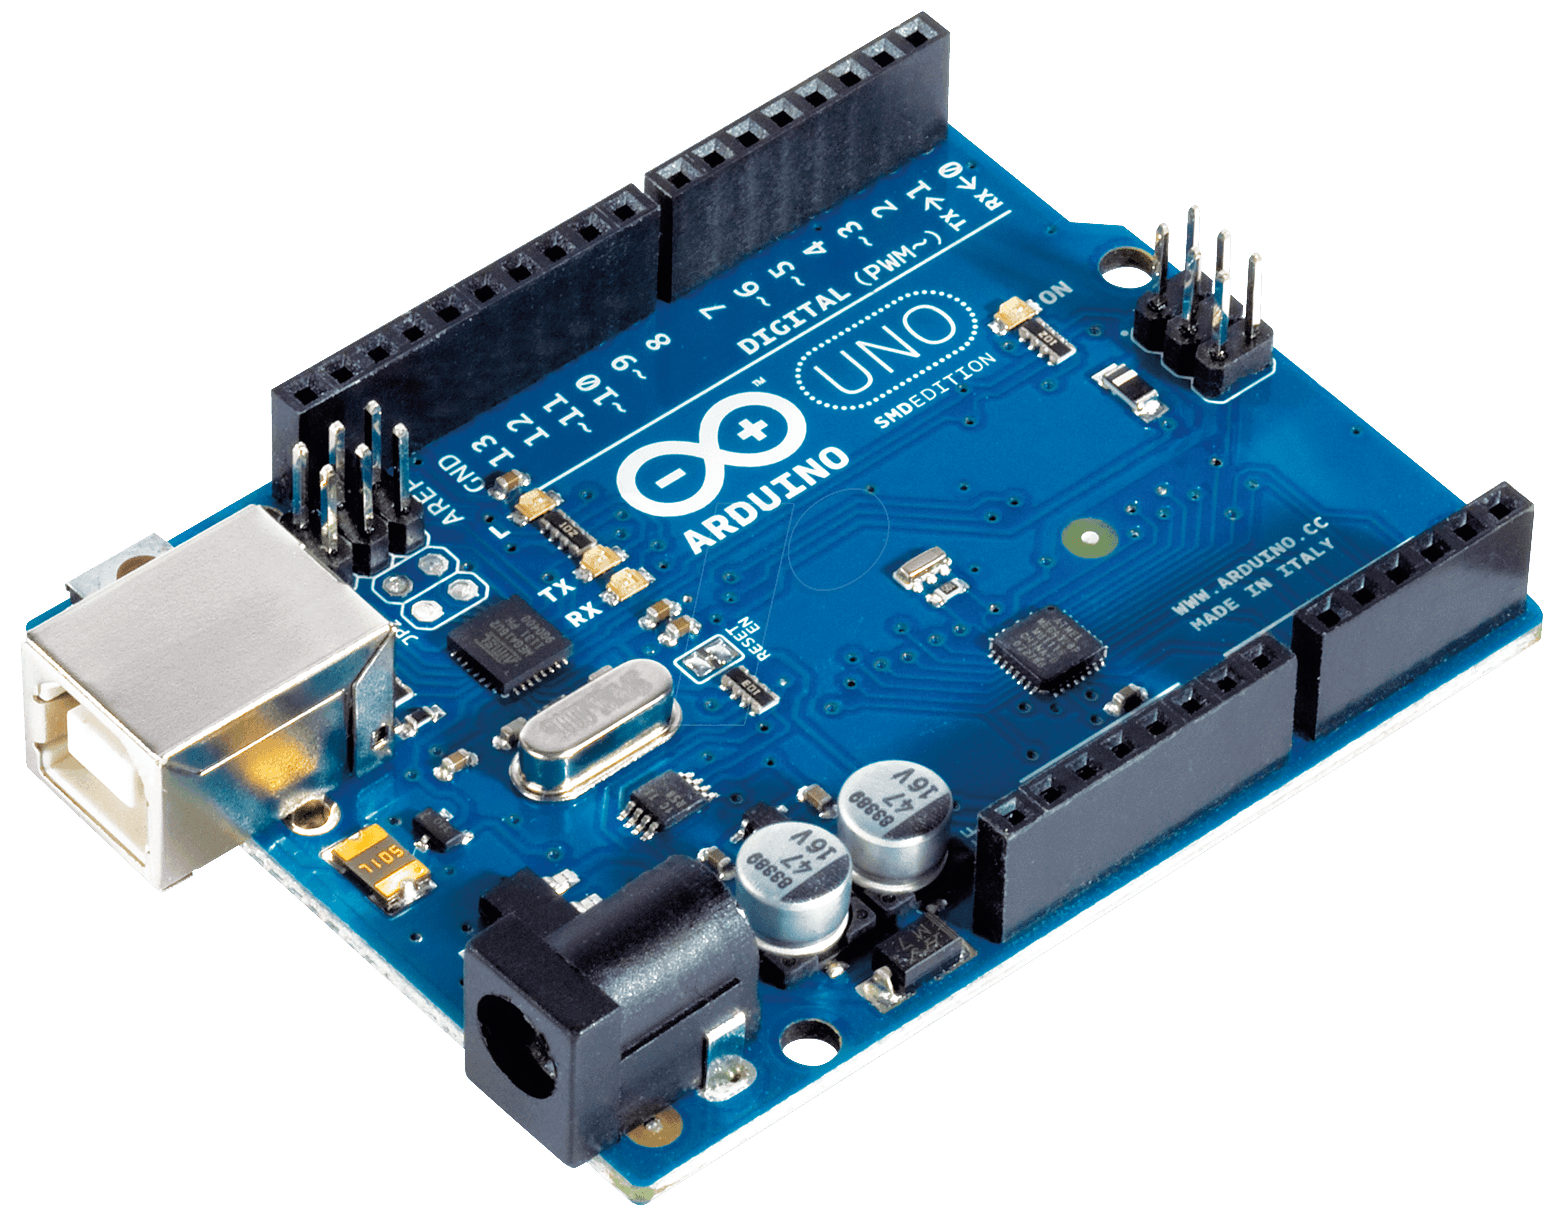
\includegraphics[width=0.75\linewidth]{ArduinoUnoR3.png}
    \caption{microcontroller: Arduino Uno R3}
    \label{fig:enter-label}
\end{figure}
Arduino Uno is a microcontroller board based on 8-bit the ATmega 328P. It has 14 digital input/output terminals, where six of them can be used as a pulse width modulation (PWM) outputs. It has six analog inputs, a 16 MHz quartz crystal,a USB connection, a power jack, and a reset button

\section{Software}
This section provides a concise overview of the software design methodology. For the full code implementation, please refer to the appendix A
The Arduino software consists of three primary components. The first component handles the acquisition of coordinate positions from the sensor. The second component deals with serial communication, enabling the exchange of data between the Arduino and the PC. Finally, the third component is devoted to the control section, managing the operational control of the system.


\subsection{Acquisition of coordinate positions}
The implementation of the algorithm for acquiring coordinate positions involves utilizing a 5-wire resistive touch screen, as illustrated in the figure 2.9.
\begin{figure}[h]
    \centering
    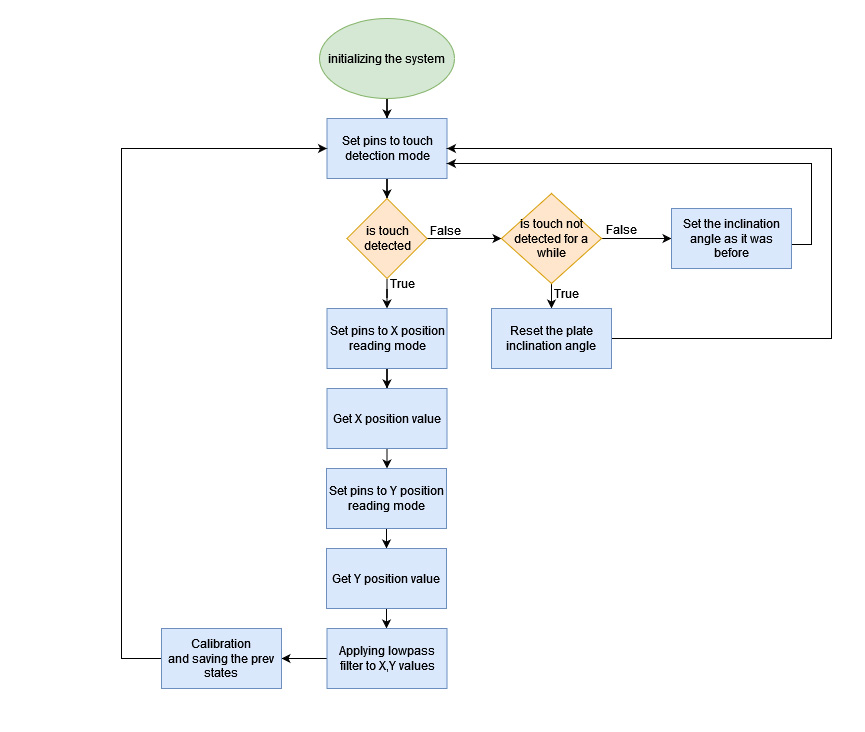
\includegraphics[width=1\linewidth]{touch_screen_algorithm_flowchart.jpg}
    \caption{Flowchart outlining the algorithm for acquiring coordinate positions from the resistive touch screen}
    \label{fig:enter-label}
\end{figure}
The flowchart illustrates the data retrieval process from the sensor, which progresses through several stages. Initially, we set the sensor to a "Stand By Mode". Upon detecting a touch on the screen, if the touch happens we instruct the sensor to capture the signal along both the X-axis and Y-axis. Subsequently, we filter the obtained readings via a lowpass filter. The figure 2.10 below demonstrates the signal's shape before and after passing through the Low-pass filter. Following the filtering, we convert the coordinates of the readings into centimeters.

\begin{figure}[h!]
    \centering
    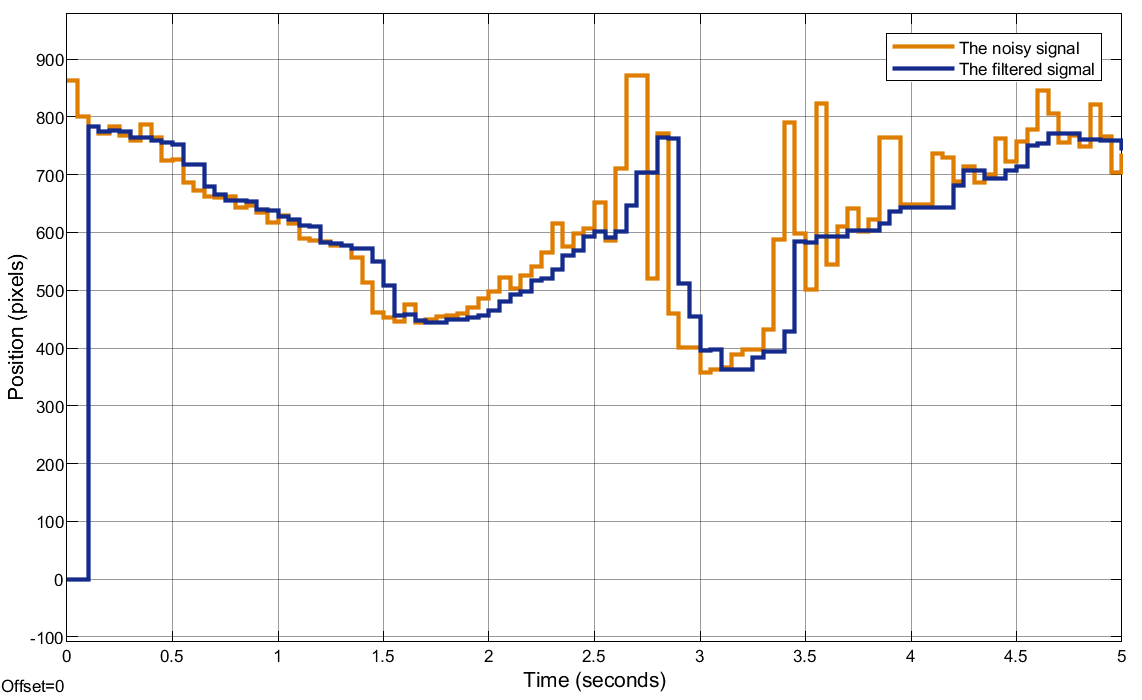
\includegraphics[width=1\linewidth]{Filter_vs_noisy_signals.png}
    \caption{Signal comparison before and after applying a low-pass filter to the resistive touch screen readings}
    \label{fig:enter-label}
\end{figure}

\subsection{Data transmission via serial communication}
Once we figure out where the ball is on plate through the Arduino, we want to share that information with the PC (Simulink). We use something called the "serial communication protocol" to send this data from the Arduino to the computer through a USB connection. Additionally, we want the computer to send back calculated output about the servomotor angle to the Arduino.

Using Instrument Control Toolbox in Simulink we could send and receive bytes in Arduino and interpret it as floats numbers, in the figure 2.11 we used Serial Configuration, Serial Send, Serial Receive blocks, cast to double block and byte pack which converts single data type to 4 packing bytes using byte alignment 4 with a header and terminator 
\begin{figure}[h!]
    \centering
    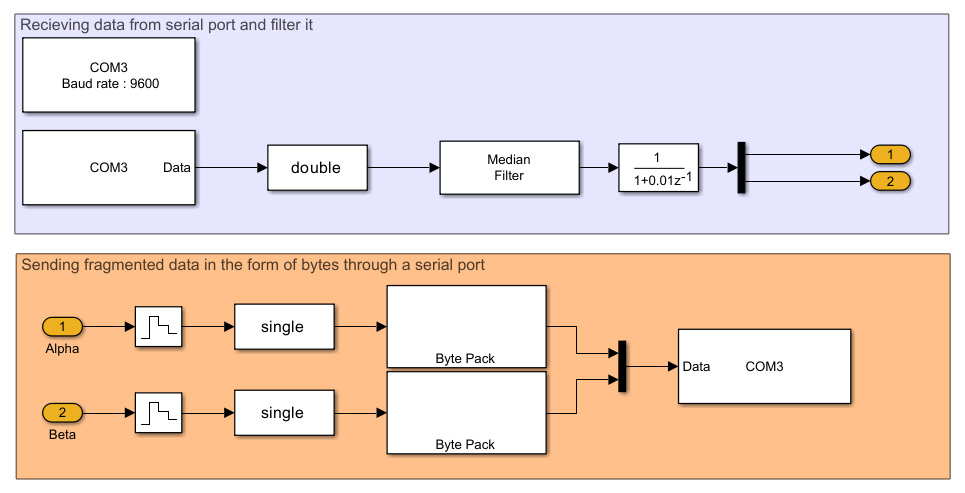
\includegraphics[width=1\textwidth]{Recieving_sending_via_serial_port.jpg}
    \caption{Serial communication setup using Simulink for data transmission between Arduino and PC}
\end{figure}

On the Arduino side, we used a union type to convert a float into an array of bytes (uint8). To receive the bytes from matlab, a function named getFloat()  was defined that converts each four bytes into float, as outlined in the code snippet presented in Figure 2.12.

\begin{figure}[h!]
    \centering
    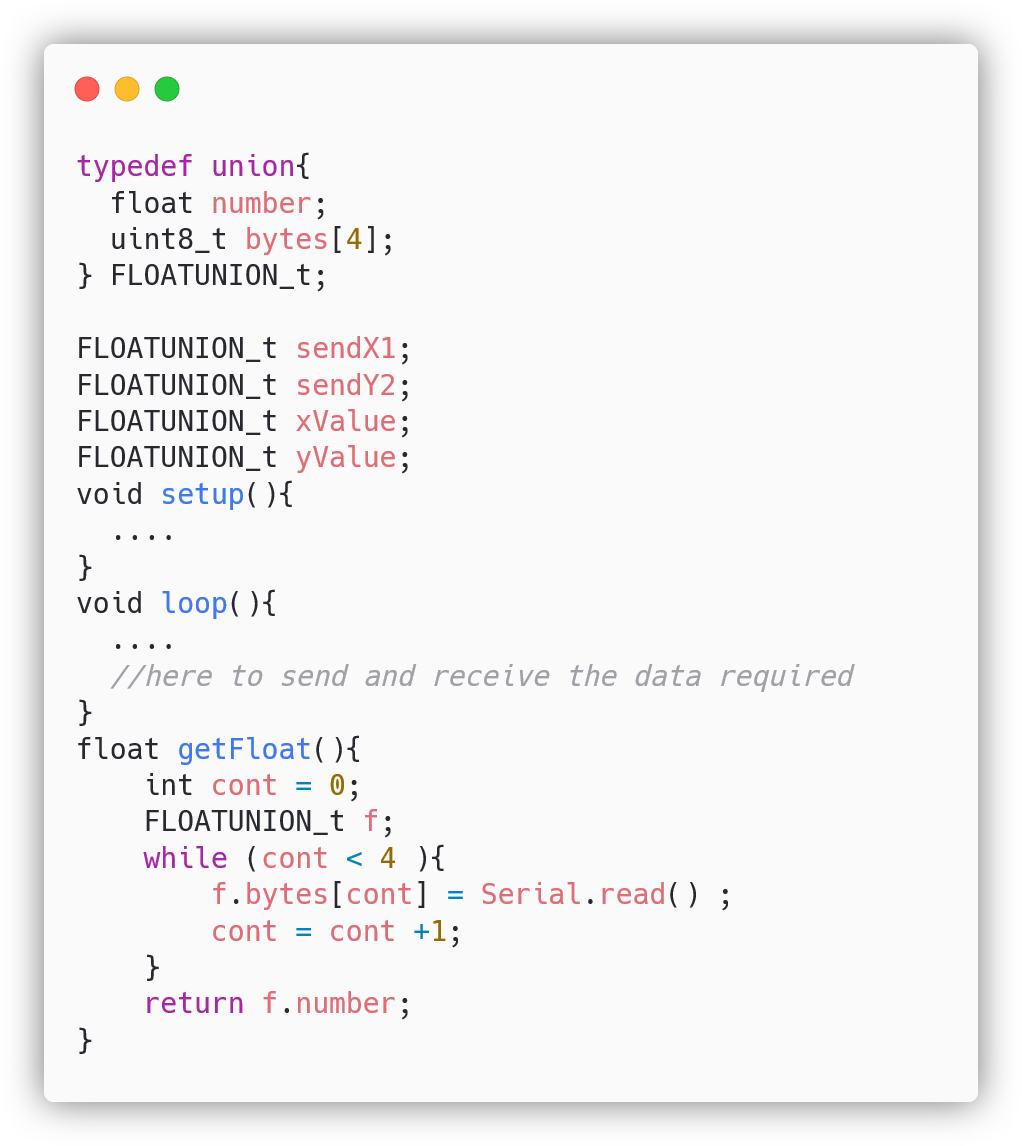
\includegraphics[width=0.8\textwidth]{carbon.png}
    \caption{Code snippet showcasing Arduino-side implementation for receiving and sending data via the serial port}
\end{figure}

\subsection{the operational control of the system}
To calculate the appropriate servomotor angle we used two methods one By by using serial communication and simulink control toolbox to control the system and the other by using the Arduino PID library designed by Brett Beauregard, in the first algorithm, the code running on the workstation communicates with the Arduino by a serial COM, therefore, the speed at which the Arduino respond is defined by the baud-rate, however the latter method is to be working in lower sampling time because there is no delay that occurs during data transfer
